\documentclass{beamer}
%
% Choose how your presentation looks.
%
% For more themes, color themes and font themes, see:
% http://deic.uab.es/~iblanes/beamer_gallery/index_by_theme.html
%
\mode<presentation>
{
  \usetheme{Madrid}      % or try Darmstadt, Madrid, Warsaw, ...
  \usecolortheme{crane} % or try albatross, beaver, crane, ...
  \usefonttheme{default}  % or try serif, structurebold, ...
  \setbeamertemplate{navigation symbols}{}
  \setbeamertemplate{caption}[numbered]
  
} 

\usepackage[english]{babel}
\usepackage[utf8x]{inputenc}
\usepackage{courier}
\usepackage{dsfont}
\usepackage{verbatim} 
\usepackage{tikz}
\usepackage{caption}
\usepackage{multirow}
\usepackage{amsmath}
\usepackage{venndiagram}
\usepackage{xcolor}
\usepackage[shortlabels]{enumitem}
\usepackage{listings}
\usepackage{hyperref}
\hypersetup{
    colorlinks=true,
    linkcolor=blue,
    filecolor=magenta,      
    urlcolor=cyan,
}
\usepackage{subfigure}

\newcommand{\code}[1]{\texttt{#1}}
\graphicspath{{img/}}

\DeclareMathOperator*{\argmax}{arg\!\max}
\DeclareMathOperator*{\argmin}{arg\!\min}
\newcommand{\vp}{\vspace{2mm}}
\newcommand{\xt}{\texttt}

\usetikzlibrary{shapes,decorations,arrows,calc,arrows.meta,fit,positioning}
\tikzset{
    -Latex,auto,node distance =1 cm and 1 cm,semithick,
    state/.style ={ellipse, draw, minimum width = 0.7 cm},
    point/.style = {circle, draw, inner sep=0.04cm,fill,node contents={}},
    bidirected/.style={Latex-Latex,dashed},
    el/.style = {inner sep=2pt, align=left, sloped}
}

\usepackage{color}
\providecommand{\pb}[1]{\textcolor{red}{#1}}
\providecommand{\cn}[1]{\textcolor{blue}{#1}}

\usepackage{listings}
\lstdefinestyle{rstyle}{
	language=R,
    %stringstyle=\color{green},
    %otherkeywords={0,1,2,3,4,5,6,7,8,9},
    %morekeywords={TRUE,FALSE},
    %deletekeywords={data,frame,length,as,character}
    %keywordstyle=\color{blue},
    %commentstyle=\color{cyan},
}

\setitemize{label=\usebeamerfont*{itemize item}%
  \usebeamercolor[fg]{itemize item}
  \usebeamertemplate{itemize item}}

\newcommand{\Mypm}{\mathbin{\tikz [x=1.4ex,y=1.4ex,line width=.1ex] \draw (0.0,0) -- (1.0,0) (0.5,0.08) -- (0.5,0.92) (0.0,0.5) -- (1.0,0.5);}}%

\title[Public Defense]{What You See is What You Get:}
\subtitle{A Closer Look at Bias in the Visual World Paradigm}
\author{Collin Nolte}
\date{March 8, 2023}

\begin{document}

\begin{frame}
  \titlepage
\end{frame}


\begin{frame}
\begin{center}
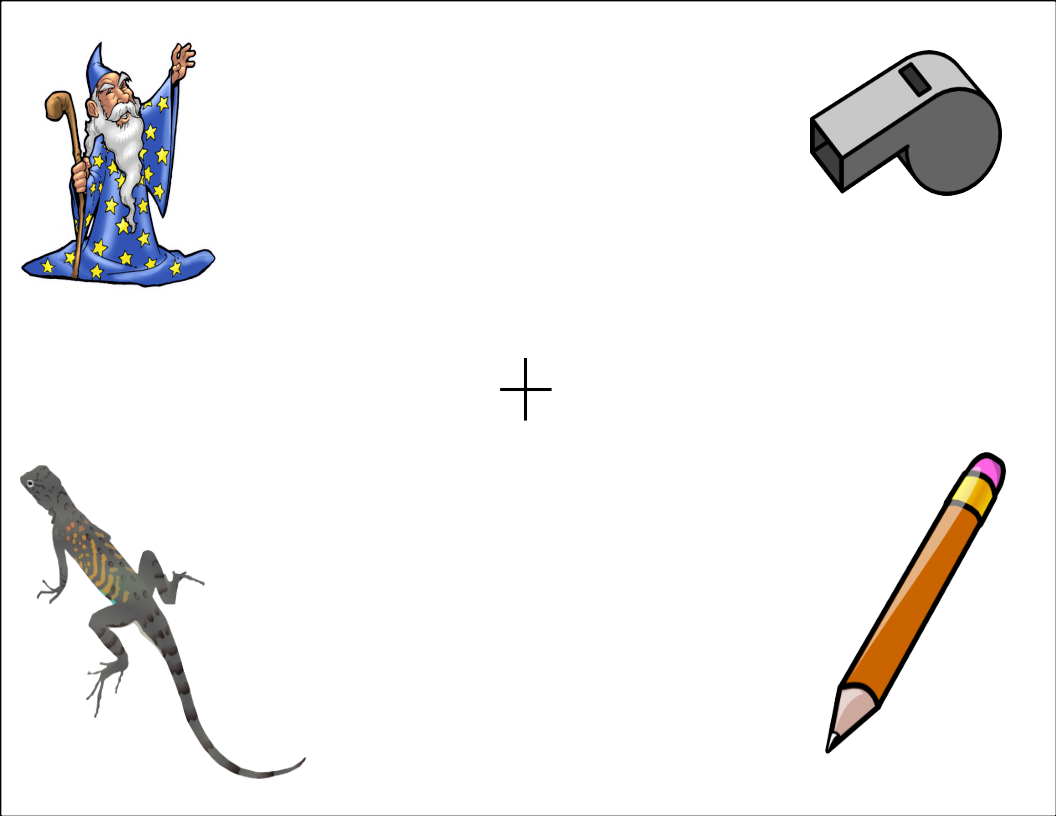
\includegraphics[scale=0.35]{img/wizard_lizard_whistle_pencil.png}
\end{center}
\end{frame}

%\begin{frame}{img (delete slide)}
%here just have a picture of a vwp trial w/o context. While the picture is up, ask some questions: 
%
%\begin{itemize}
%\item what are some images on screen? any obvious relations? (rhymes, begin same)
%\item If I told you to look at the wizard, how might i be able to tell when you understand exactly what I meant? (hopefully they answer eyes)
%\item what are some things i should be aware of when considering eyes (scanning, back and forth, etc)
%\end{itemize}
%\end{frame}


% language and cognition
\begin{frame}{Language and Cognition}\large
The field is itself exceptionally broad, ranging from sentence processing, priming, reading, and word formation \vspace{4mm}

%\begin{center}
%``trink" $\Rightarrow$ ``trank" or ``trinked"? \vp
%\end{center}

Troublesome when we commit too early: \vp

\begin{center}
``The horse raced past the barn fell"  \vspace{4mm}
\end{center}

Often can not be observed directly  \vspace{4mm}

Limit focus to single word recognition 



%This is such a seriously huge topic ranging from word recognition to sentence comprehension \\
%This also extends to thinks like reading \\
%Here, we are going to limit our consideration to single word recogntion \\
%It all starts with an audio signal that is interpreted by our brains in real time
\end{frame}

% cohort illustration

\begin{frame}
\begin{center}
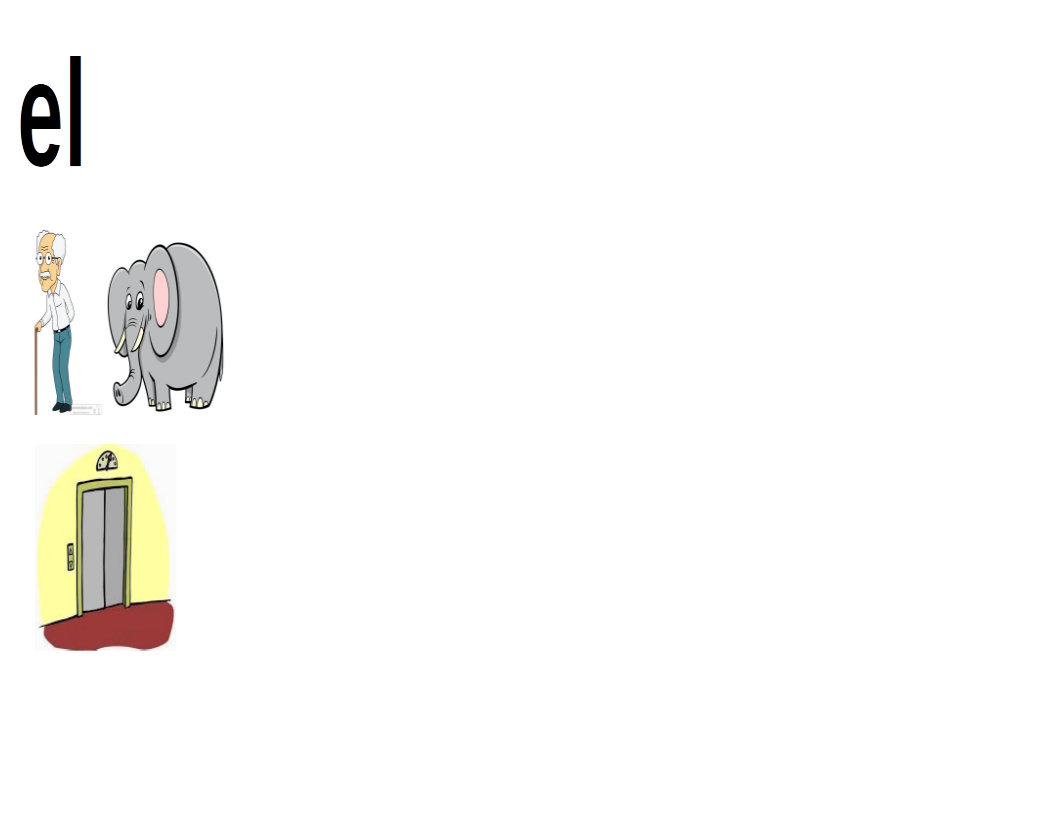
\includegraphics[scale=0.3]{img/ele_1.png}
\end{center}
\end{frame}

\begin{frame}
\begin{center}
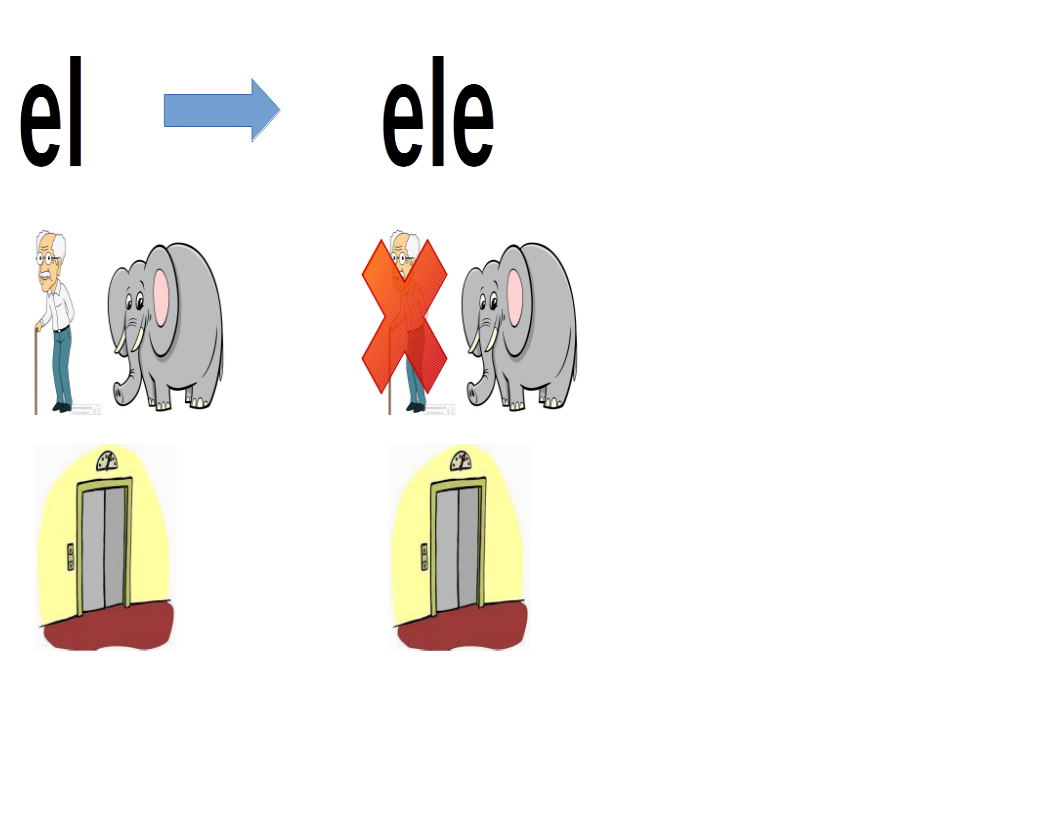
\includegraphics[scale=0.3]{img/ele_2.png}
\end{center}
\end{frame}

\begin{frame}
\begin{center}
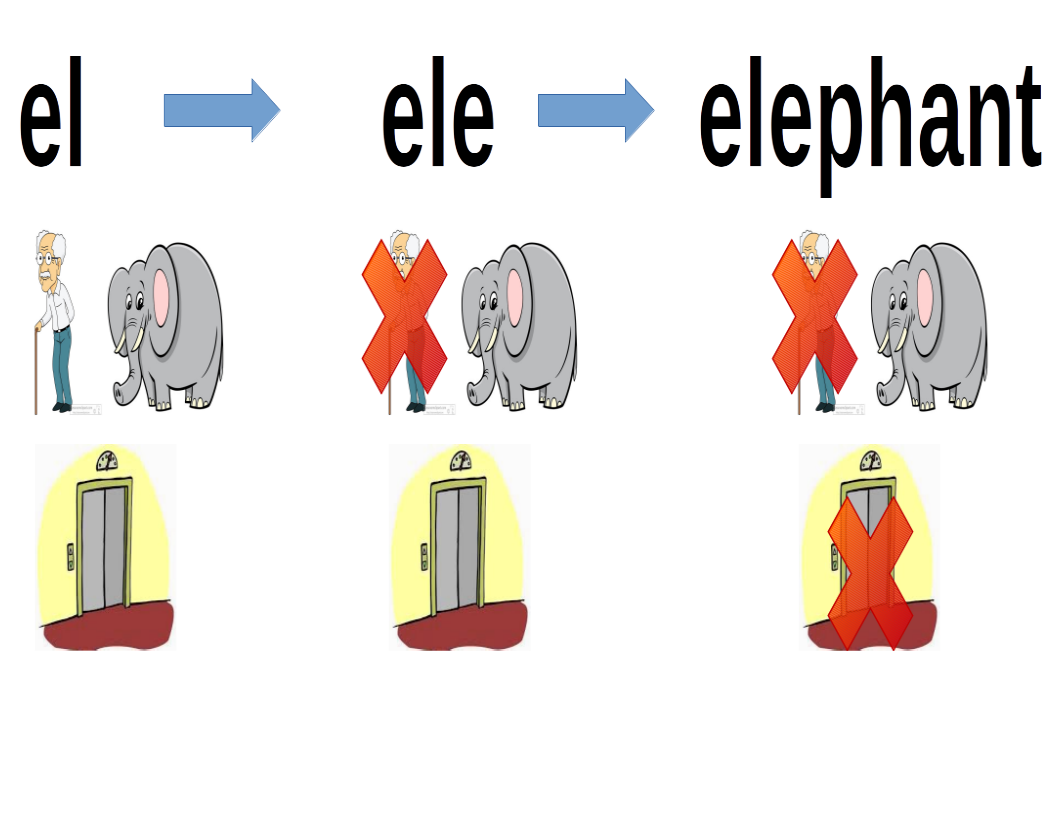
\includegraphics[scale=0.3]{img/ele_3.png}
\end{center}
\end{frame}


%
%\begin{frame}{How does this evolve in time?} \large
%Continuous mapping models of word recognition account for variety of observed phenomenon  \vp
%
%\cn{things like immediacy (hypothesis formed from earliest input), parallelism (multiple items activated, i.e., priming), graded activation (not all-or-nothing)} \vp
%
%In particular, connectionist models of lexical access (such as TRACE):
%\begin{itemize}
%\item Network structure \cn{relies on information between levels, i.e., phonemes, words, etc.)}
%\item Processes in real time \cn{along with network structure, accommodates competition}
%\item Nodes, activation, and signal \cn{metaphors that motivate language used to describe it}
%\end{itemize}
%\end{frame}
%
%
%
%% what does trace look like
%\begin{frame}
%\begin{center}
%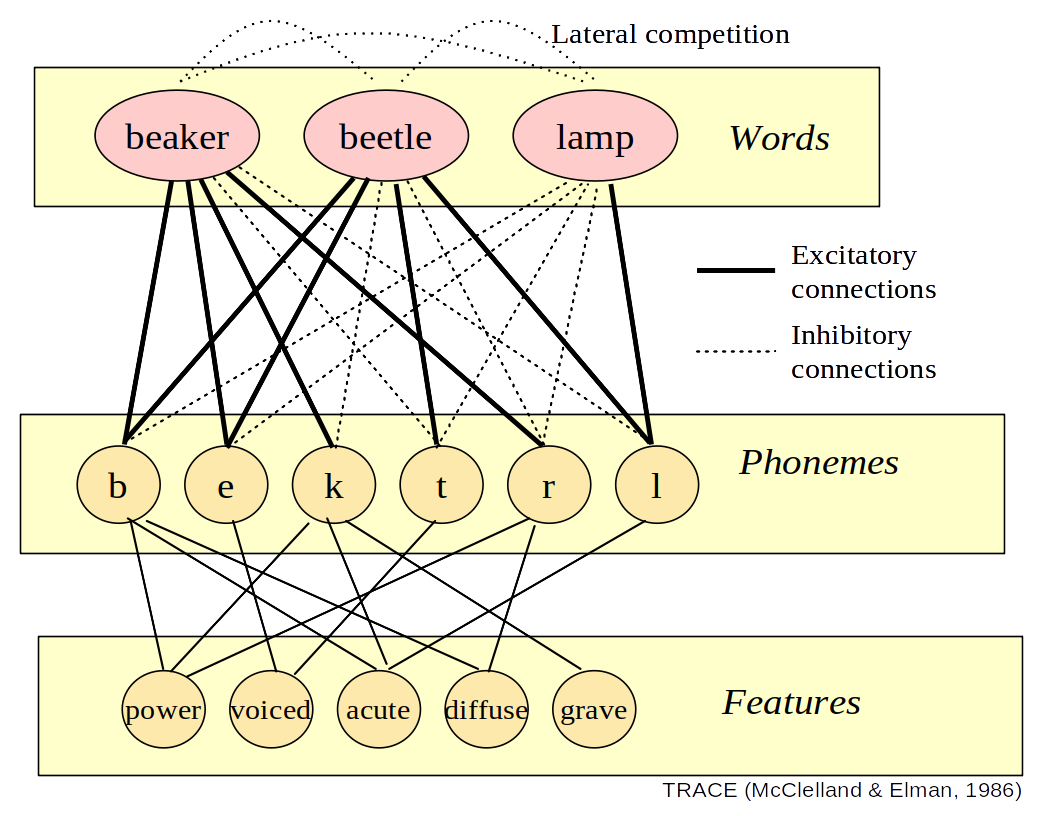
\includegraphics[scale=0.4]{img/trace_competition.png}
%\end{center}
%\end{frame}
%
%\begin{frame}
%\begin{figure}
%\centering
%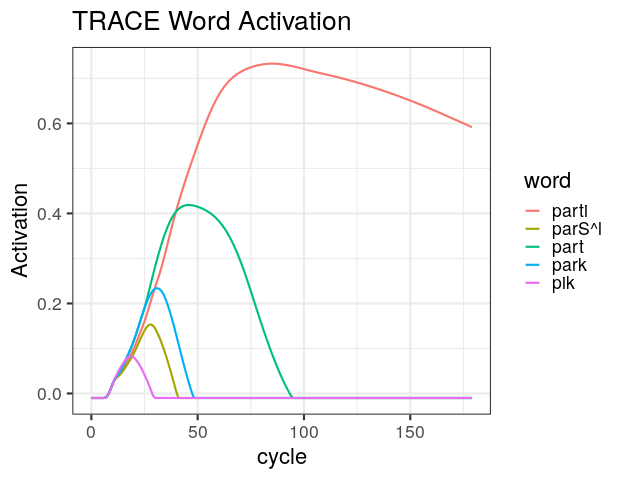
\includegraphics[scale=0.5]{img/trace_plot.png}
%\caption{gave up on reordering the legend}
%\end{figure}
%\end{frame}

\begin{frame}
\begin{figure}
\centering
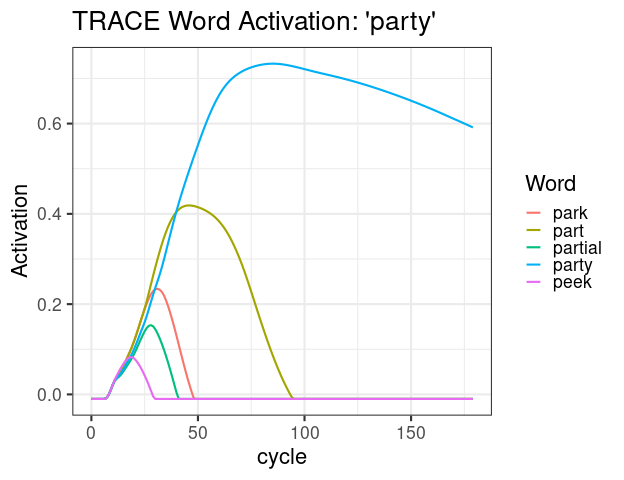
\includegraphics[scale=0.5]{img/trace_plot_reg.png}
\end{figure}
\end{frame}


% why is this important?
\begin{frame}{Why do we care?}

Typically interested in comparing activation between groups or conditions \vspace{2mm}

\begin{itemize}
\item Normal Hearing (NH) vs Cochlear Implants (CI) \vspace{2mm}
\item Differentiating cognitive, specific, and non-specific impairments \vspace{2mm}
\end{itemize}

How do we measure this?


\end{frame}


\begin{frame}%{What's in a look?}
\vspace{-1mm}
\begin{figure}
\centering
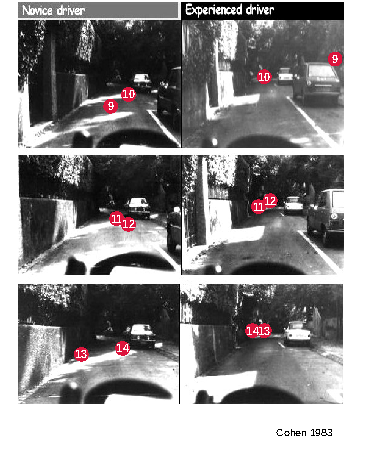
\includegraphics[scale=1.32]{img/edit_car_eye.pdf}
\end{figure}
\end{frame}



%\begin{frame}{Visualizing Eye Mechanics}
%\vspace{-1mm}
%\begin{figure}
%\centering
%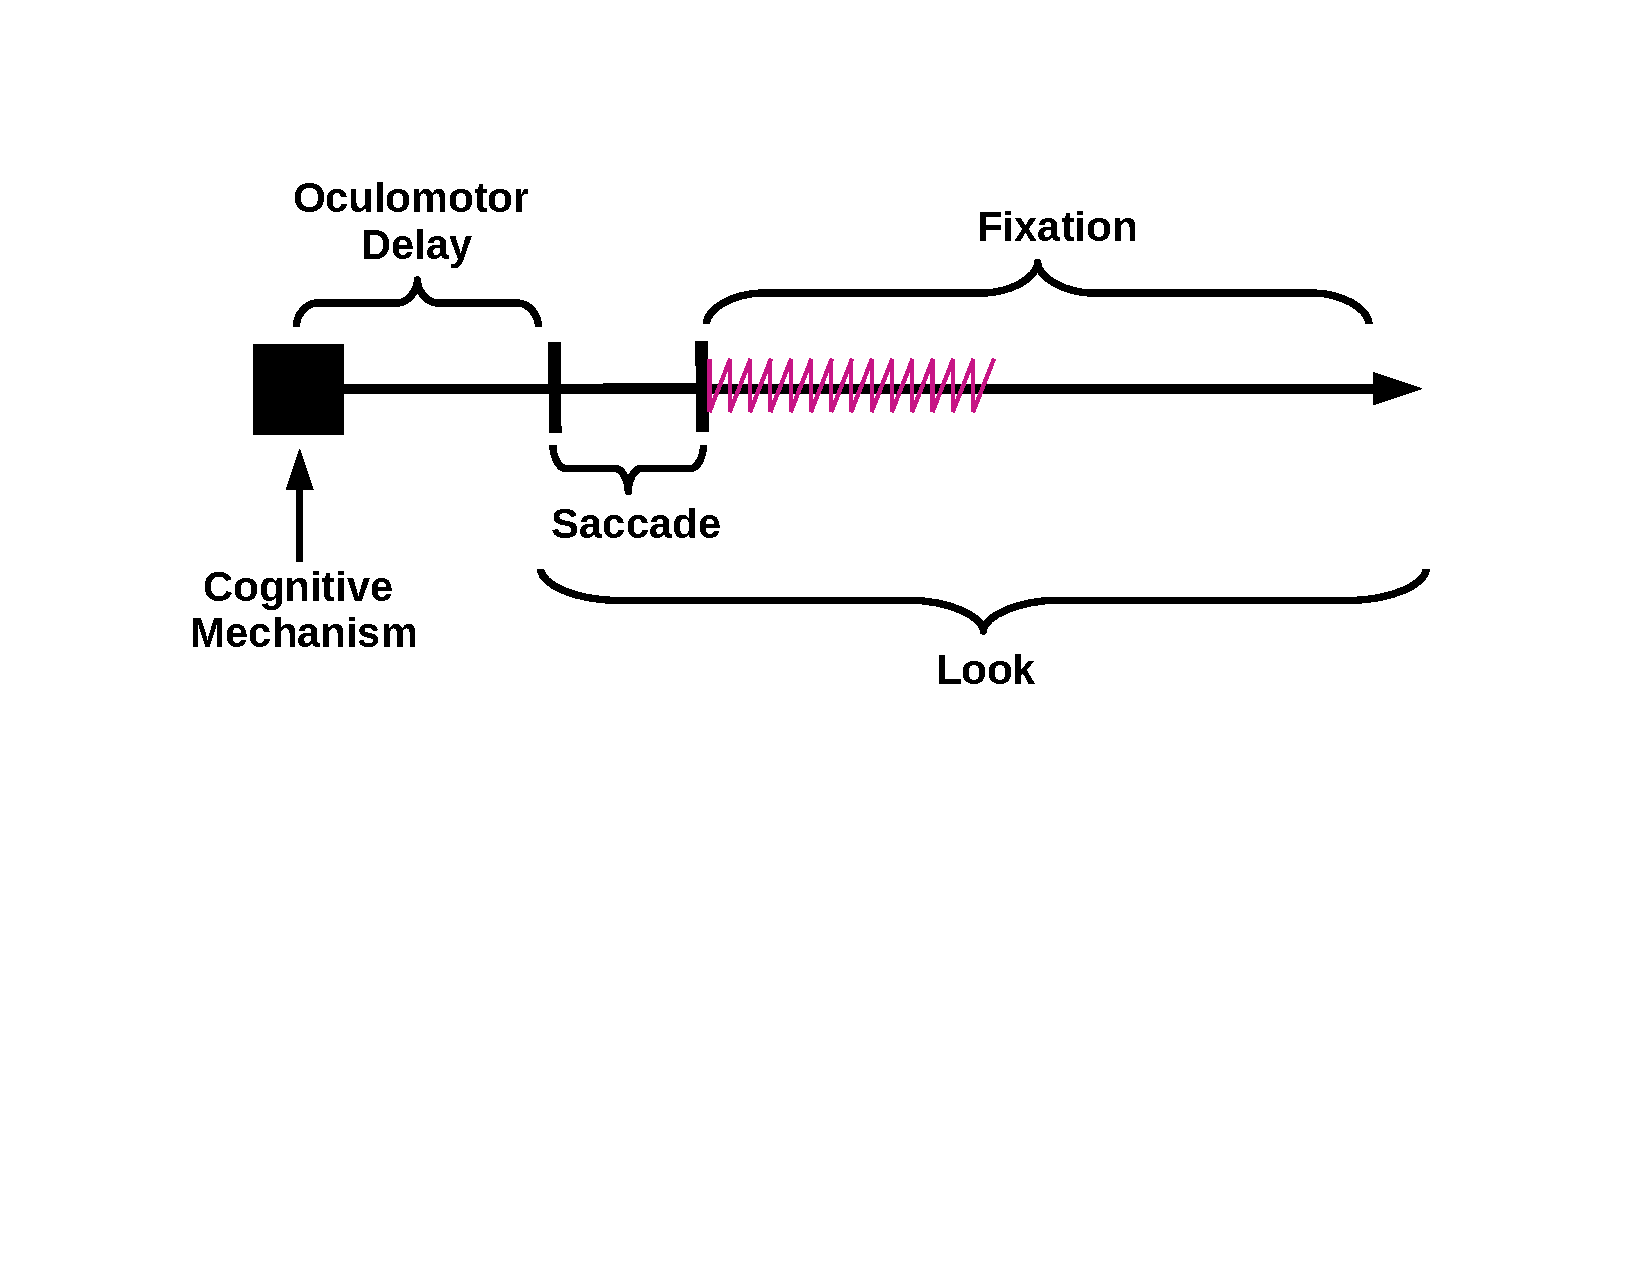
\includegraphics[scale=0.45]{img/what_is_a_look.pdf}
%\caption{just describe this with words, mention 200ms delay, etc)}
%\end{figure}
%\end{frame}




% Enter vwp
\begin{frame}{Visual World Paradigm}\large
\begin{columns}
\begin{column}{0.45\textwidth}

Visual World Paradigm (VWP) introduced in 1995 \vspace{4mm}

Eye tracking in conjunction with spoken sentence  \vspace{4mm}

``Put the apple on the towel in the box" 


\end{column}
\begin{column}{0.5\textwidth}  %%<--- here
\begin{center}
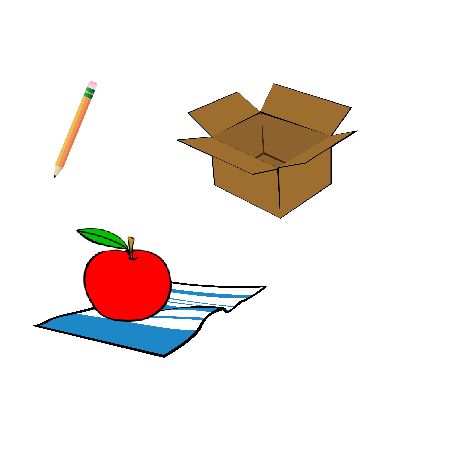
\includegraphics[scale=.9]{img/towel_apple_box.pdf}
\end{center}
\end{column}
\end{columns}
\end{frame}

%\begin{frame}{alt image for vwp}
%\vspace{-3mm}
%\begin{figure}
%\centering
%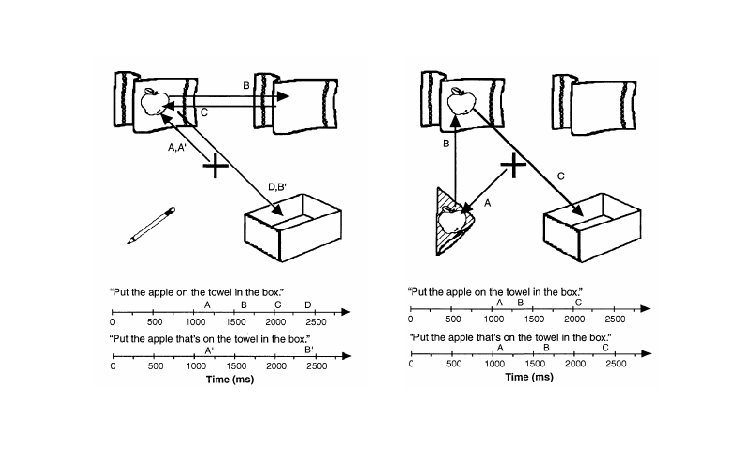
\includegraphics[width=\textwidth]{apple_combine.pdf}
%%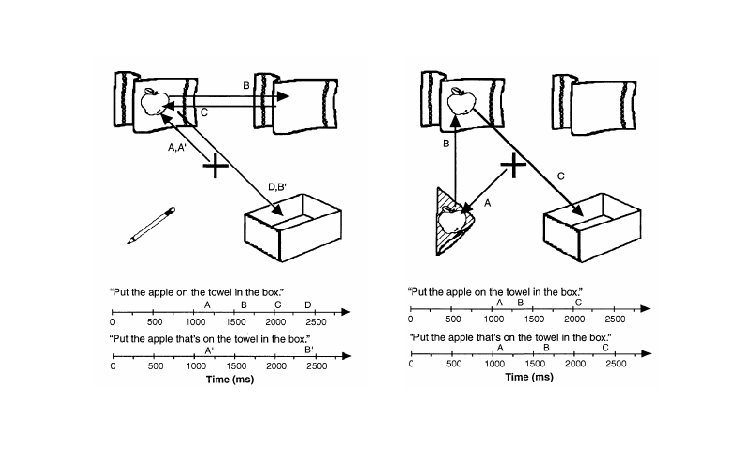
\includegraphics[scale = 1.1]{apple_combine.pdf}
%\caption{Differential eye response based on context and ambiguity}
%\end{figure}
%\end{frame}

\begin{frame}%{alt image for vwp}
\begin{figure}
\centering
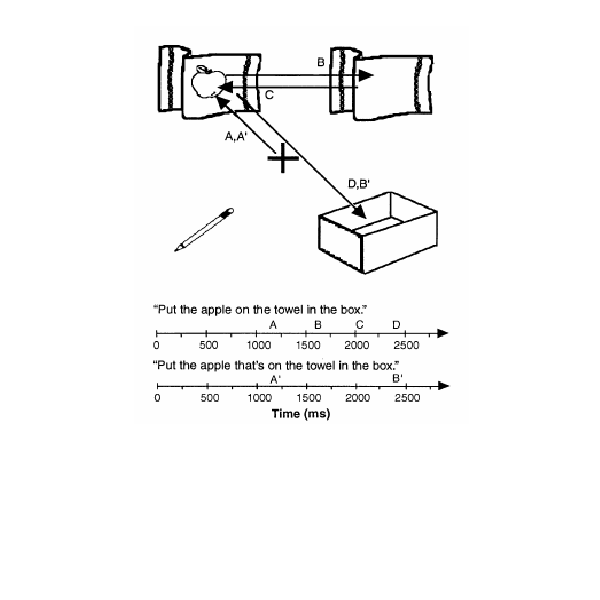
\includegraphics[width=\textwidth]{apple_combine_half.pdf}
%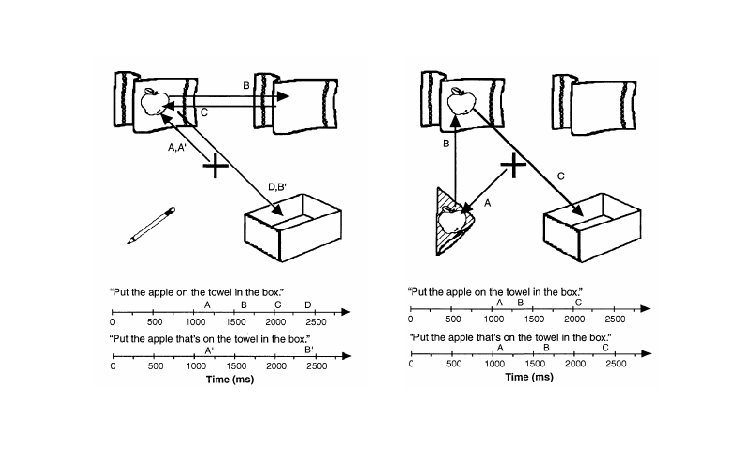
\includegraphics[scale = 1.1]{apple_combine.pdf}
\caption{Differential eye response based on context and ambiguity}
\end{figure}
\end{frame}


\begin{frame}{Outline}\large


\begin{itemize}
	\item Eye tracking and the VWP \vp
	\item Methodology 
	\begin{itemize}
	\item Proportion of Fixations Method
	\item Bias
	\item Look Onset Method \vp
	\end{itemize}
	\item Simulation
\end{itemize}

\end{frame}




\begin{frame}{VWP Trials}
\begin{center}
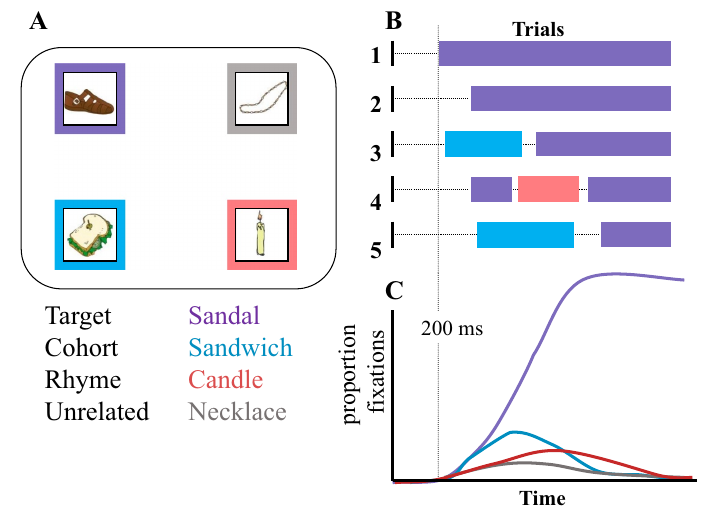
\includegraphics[scale=0.4]{img/bob_vwp_full.png}
\end{center}
\end{frame}

% just image from allopenna, magnuson and tanenhaus 
%\begin{frame}{Eye tracking as activation}
%\begin{center}
%% screenshot from paper
%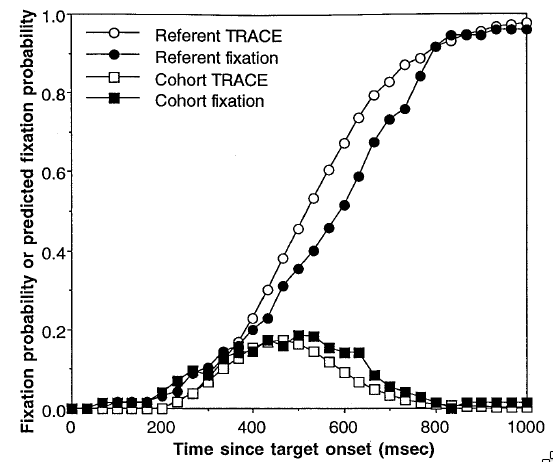
\includegraphics[scale=0.45]{img/allopenna_trace_compare.png}
%\end{center}
%\end{frame}

\begin{frame}%{Eye tracking as activation}
\begin{center}
% screenshot from paper
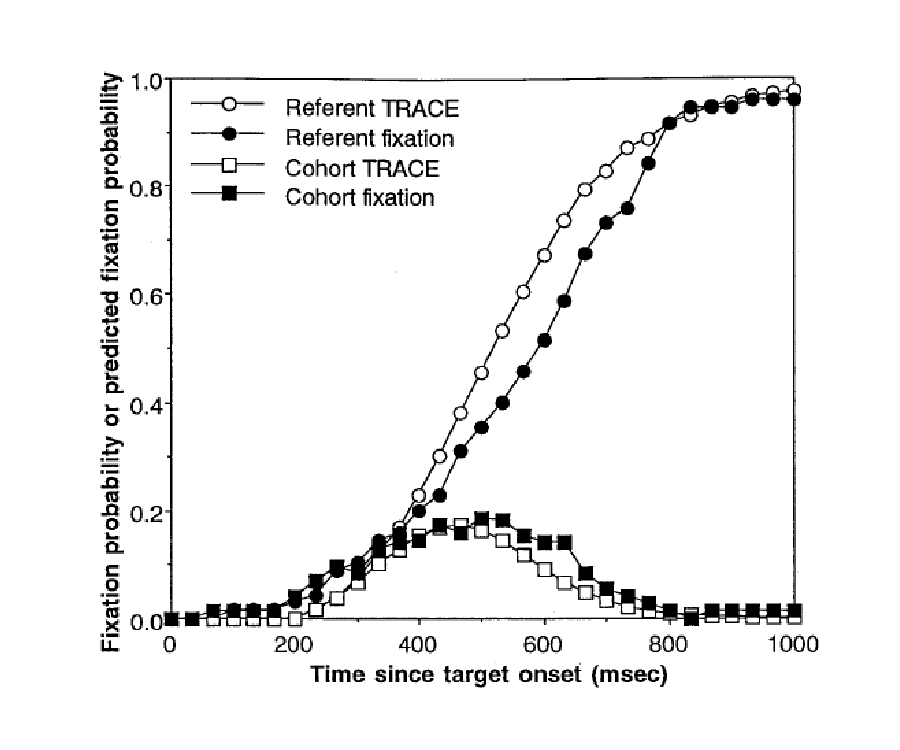
\includegraphics[scale=.75]{img/trace_compare_edit.pdf}
\end{center}
\end{frame}


% how related to vwp
\begin{frame}{So how does this relate to VWP}

\begin{columns}
\begin{column}{0.45\textwidth}

``Proportion of fixations" method \vp

Letting $z_{jt}$ represent an indicator of fixation at time $t$ for trial $j = 1, \dots, J$, we have empirical curve
\begin{align*}
y_{t} = \frac1J \sum_j z_{jt}
\end{align*}
and find
\begin{align*}
\hat{\theta} = \argmin_{\theta} \mathcal{L}(f_{\theta}, y)
\end{align*}

\end{column}
\begin{column}{0.5\textwidth}  %%<--- here
\begin{center}
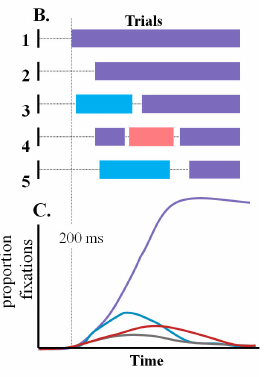
\includegraphics[scale=0.5]{img/bob_aggregate.png}
\end{center}
\end{column}
\end{columns}
\end{frame}

\begin{frame}{Proportion of Fixation Data}

\begin{columns}
\begin{column}{0.6\textwidth}
\begin{table}[ht]
\centering
\begin{tabular}{ccc|ccc}
\multicolumn{6}{c}{Fixation Trial Data} \\ 
& \\
  \hline
Trial & $t$ & Target & Trial & $t$ & Target \\ 
  \hline
  1 &   0 &   0 &   2 &   0 &   1 \\ 
    1 &   4 &   0 &   2 &   4 &   1 \\ 
    1 &   8 &   0 &   2 &   8 &   1 \\ 
    1 &  12 &   0 &   2 &  12 &   1 \\ 
    1 &  16 &   0 &   2 &  16 &   1 \\ 
    \vdots &  \vdots &   \vdots &   \vdots &  \vdots &   \vdots \\ 
    1 & 1596 &   1 &   2 & 1596 &   1 \\ 
    1 & 1600 &   1 &   2 & 1600 &   1 \\ 
   \hline
\end{tabular}
\end{table}
\end{column}

\begin{column}{0.1\textwidth}  %%<--- here
\centering
{\huge $\Rightarrow$}
\end{column}

\begin{column}{0.3\textwidth}  %%<--- here
\vspace{5mm}
\begin{table}[ht]
\centering
\begin{tabular}{cc}
\multicolumn{2}{c}{Proportion Data} \\ 
& \\
  \hline
$t$ & Target \\ 
  \hline
  0 & 0.00 \\ 
    4 & 0.01 \\ 
    8 & 0.02 \\ 
   12 & 0.02 \\ 
   16 & 0.04 \\ 
   \vdots & \vdots \\ 
  1596 & 0.91 \\ 
  1600 & 0.92 \\ 
   \hline
\end{tabular}
\end{table}
\end{column}
\end{columns}



\end{frame}


\begin{frame}{Target -- Logistic}

\vspace{-5mm}

\begin{columns}
\begin{column}{0.45\textwidth}

\begin{align*}
f(t | \theta) = b + \frac{p-b}{1 + \exp \left( \frac{4s}{p-b} (c - t) \right)}
\end{align*}
%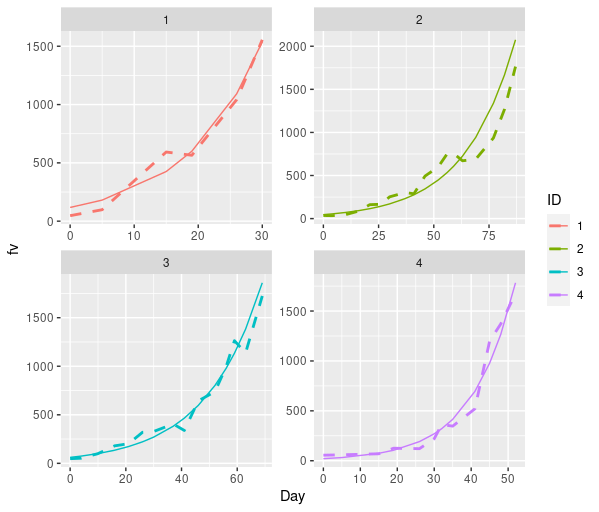
\includegraphics[scale=0.45]{img/tumr_fit.png}
\end{column}
\begin{column}{0.5\textwidth}  %%<--- here
\begin{center}
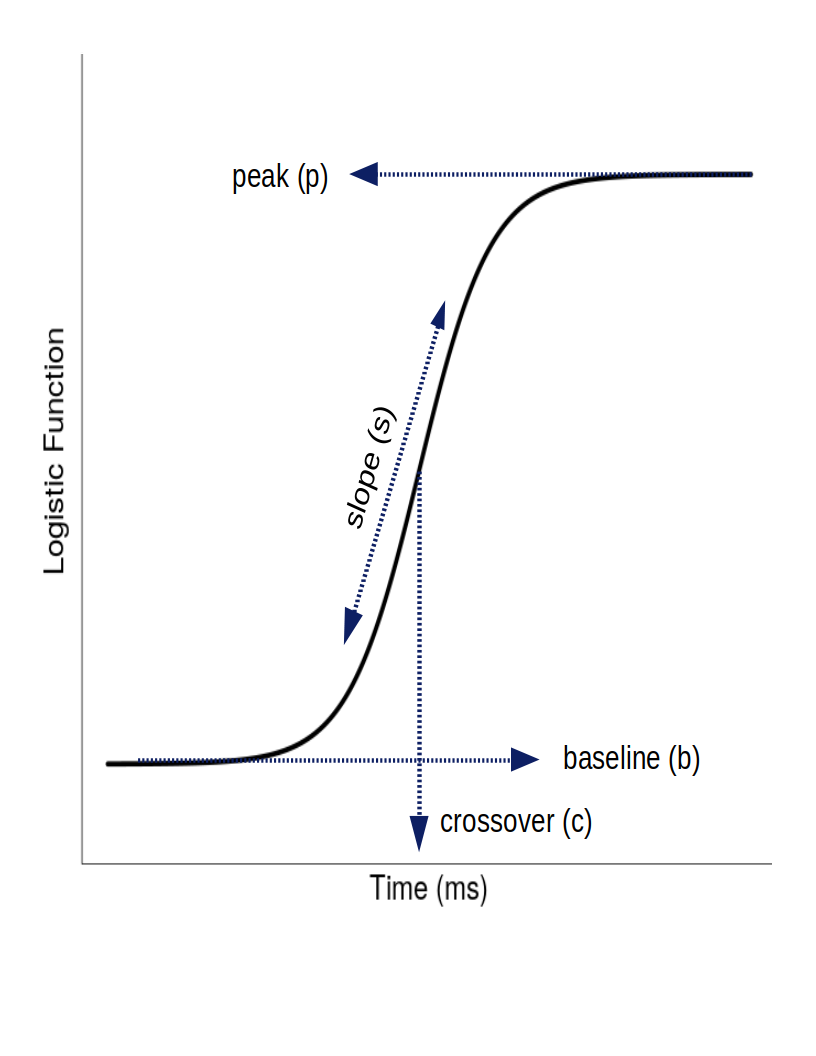
\includegraphics[scale=0.3]{img/logistic_label.png}
\end{center}
\end{column}
\end{columns}
\end{frame}
%
\begin{frame}
\begin{center}
\centering
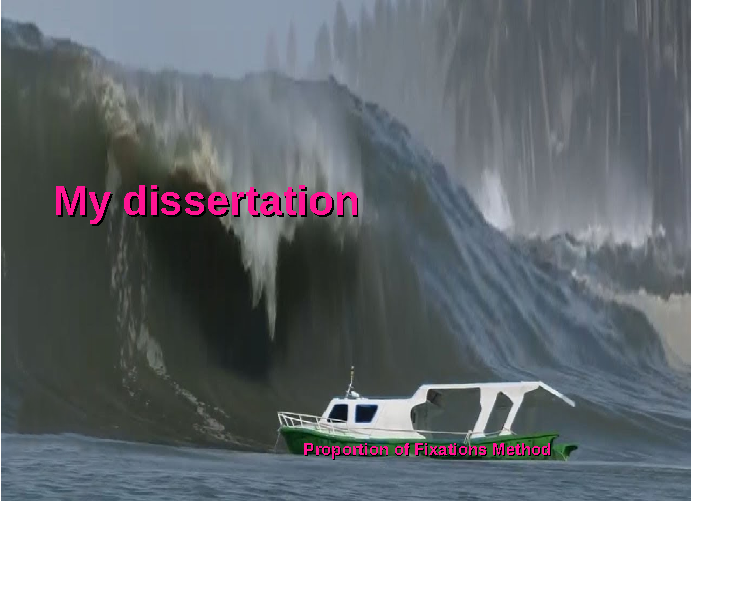
\includegraphics[scale=1]{boat_meme.pdf}
\end{center}
\end{frame}

%\begin{frame}
%\begin{center}
%%\centering
%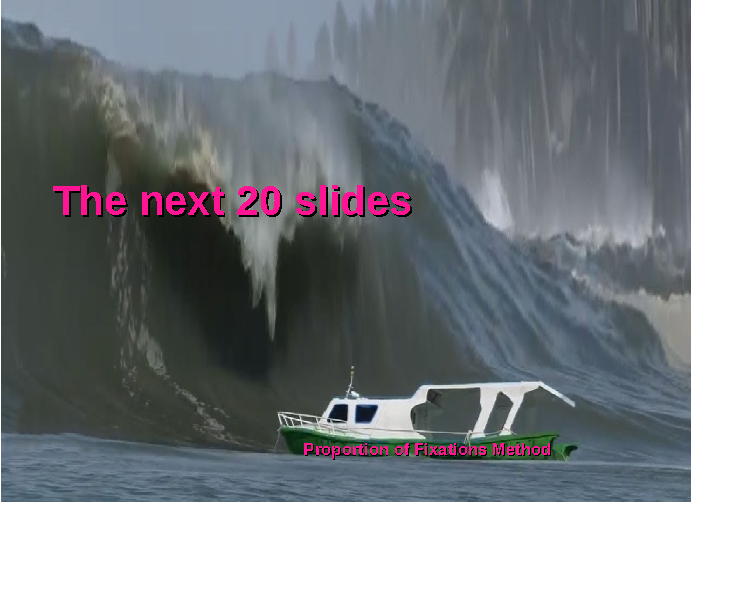
\includegraphics[scale=1]{other_boat_meme.pdf}
%\end{center}
%\end{frame}
%

%\begin{frame}{Linking hypothesis}\Large
%
%Have used $f(t|\theta)$ as functional form for proportion of fixations, but relation to activation still implicit/undefined \vp
%
%
%
%Our primary proposal is that it is the underlying activation, rather than observed data, that should be modeled explicitly as $f(t|\theta)$ \vp
%
%%Under this proposal, there are major issues with proportion of fixation method
%
%\end{frame}

\begin{frame}{Issues}\large



Despite visual similarities between the proportion of fixations, $y_t$ and lexical activation $f$, there is an issue with the equivalence \vspace{6mm}


Eye mechanics made up of distinct mechanisms that are differentially related to activation 


\end{frame}

\begin{frame}{Visualizing Eye Mechanics}
\vspace{-1mm}
\begin{figure}
\centering
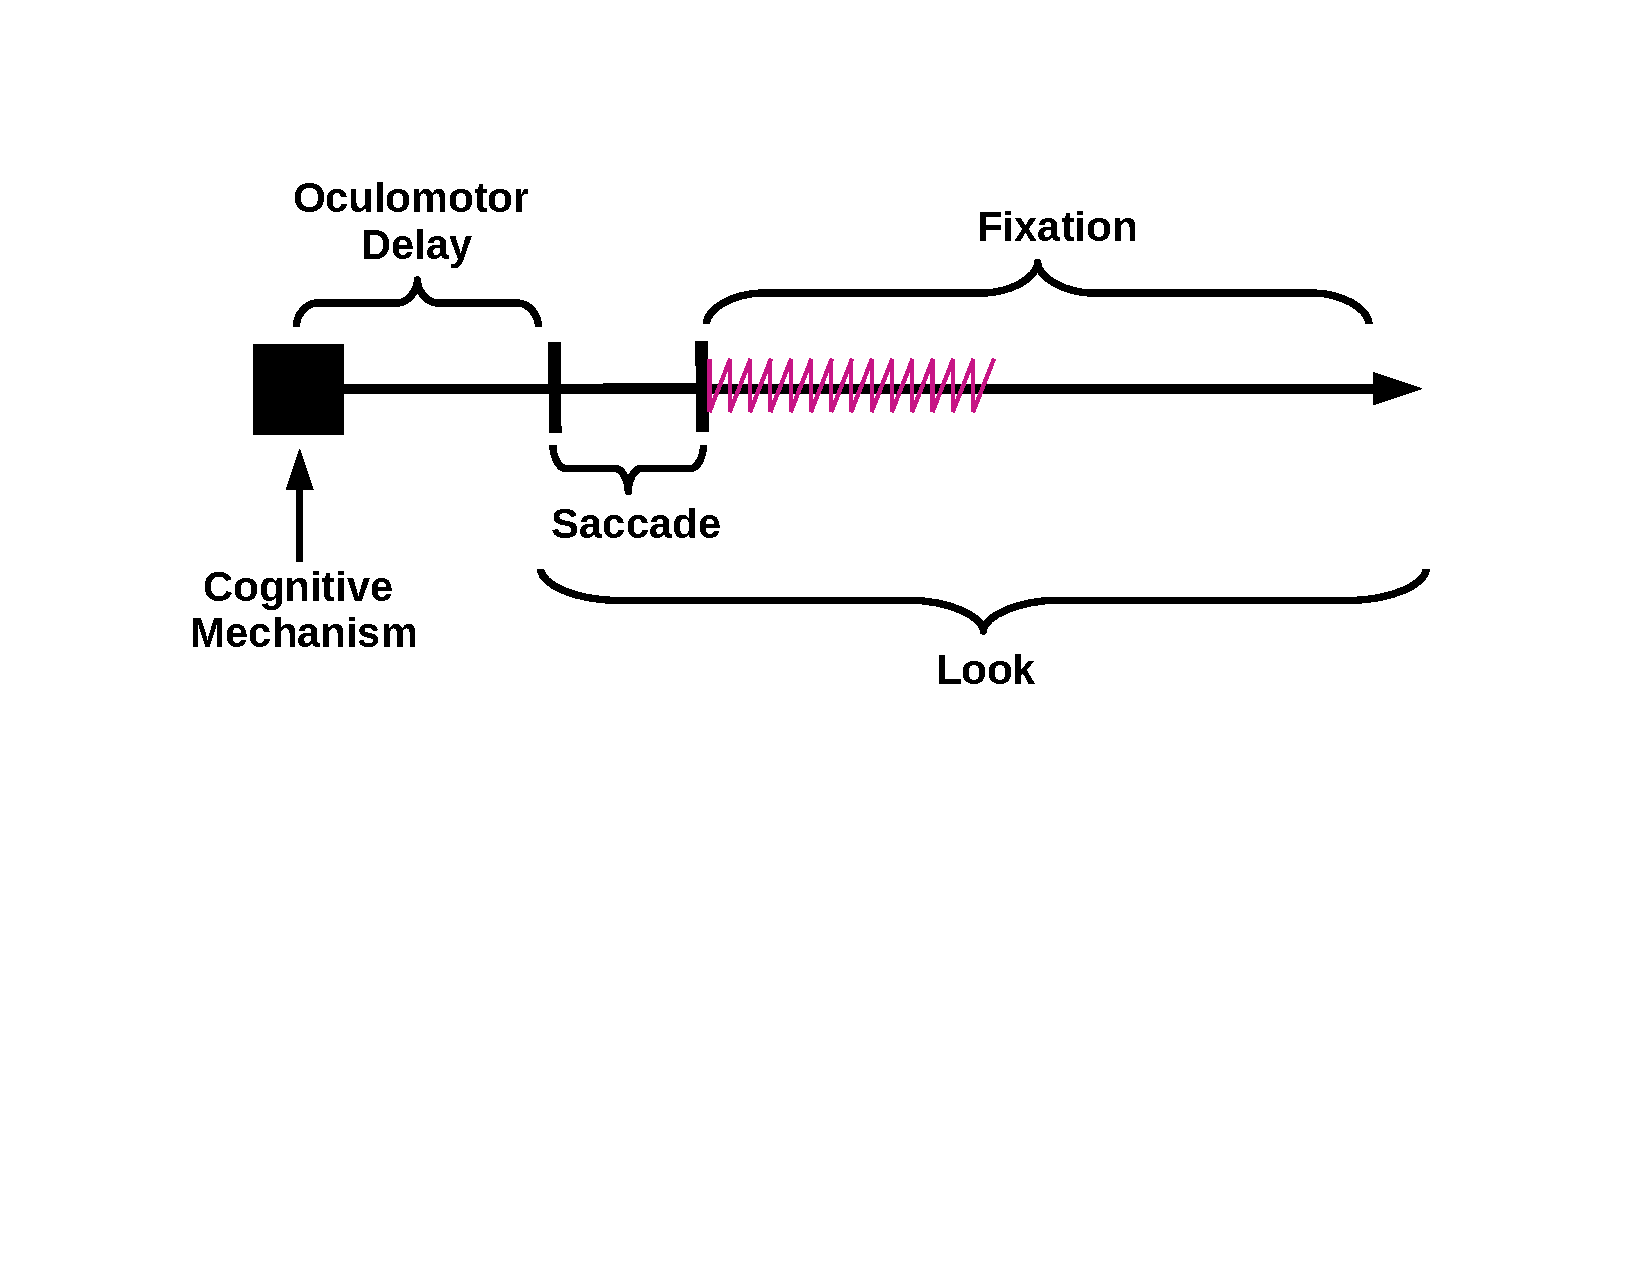
\includegraphics[scale=0.45]{img/what_is_a_look.pdf}
\end{figure}
\end{frame}


%
%\begin{frame}{Issues (another attempt)}
%We are predominately interested in the recovery of a lexical activation function, though given visual similarities between the proportion of fixations and activation, we have the ostensible equivalence, 
%
%\begin{equation}
%y_{it} \equiv f(t | \theta_i)
%\end{equation}
%
%There are primarily two sources of biases inherent in this method which hitherto have been left unexamined:
%
%\begin{itemize}
%\item[1.] Delayed observation bias/error
%\item[2.] Added observation bias
%\end{itemize}
%
%\cn{(in reverse order because easier to explain plus its mostly an aside)}
%\end{frame}


\begin{frame}{Added Observation Bias}\large

There are two primary sources of bias to address

\begin{itemize}
\item Added observation bias
\item Oculomotor delay
\end{itemize}

\vspace{6mm}

Added observation bias arises from the conflation of two distinct (though likely correlated) processes: the decision to initiate an eye movement to a particular place and the duration of a fixation 
%
%\cn{We are interested in the process that probabilistically determines the \textit{location} of a fixation} \vp
%
%\cn{At some time $t$, a saccade is launched, and we know from length of saccade until \textit{at least} refractory period for fixation, it is impossible for our eyes to go anywhere else} \vp

%By including the entire length of the fixation as ``observed" data relating to this process, we are both inflating the amount of data we have with data that is necessarily biased
\end{frame}


\begin{frame}{Activation curve}
\vspace{-5mm}
\begin{center}
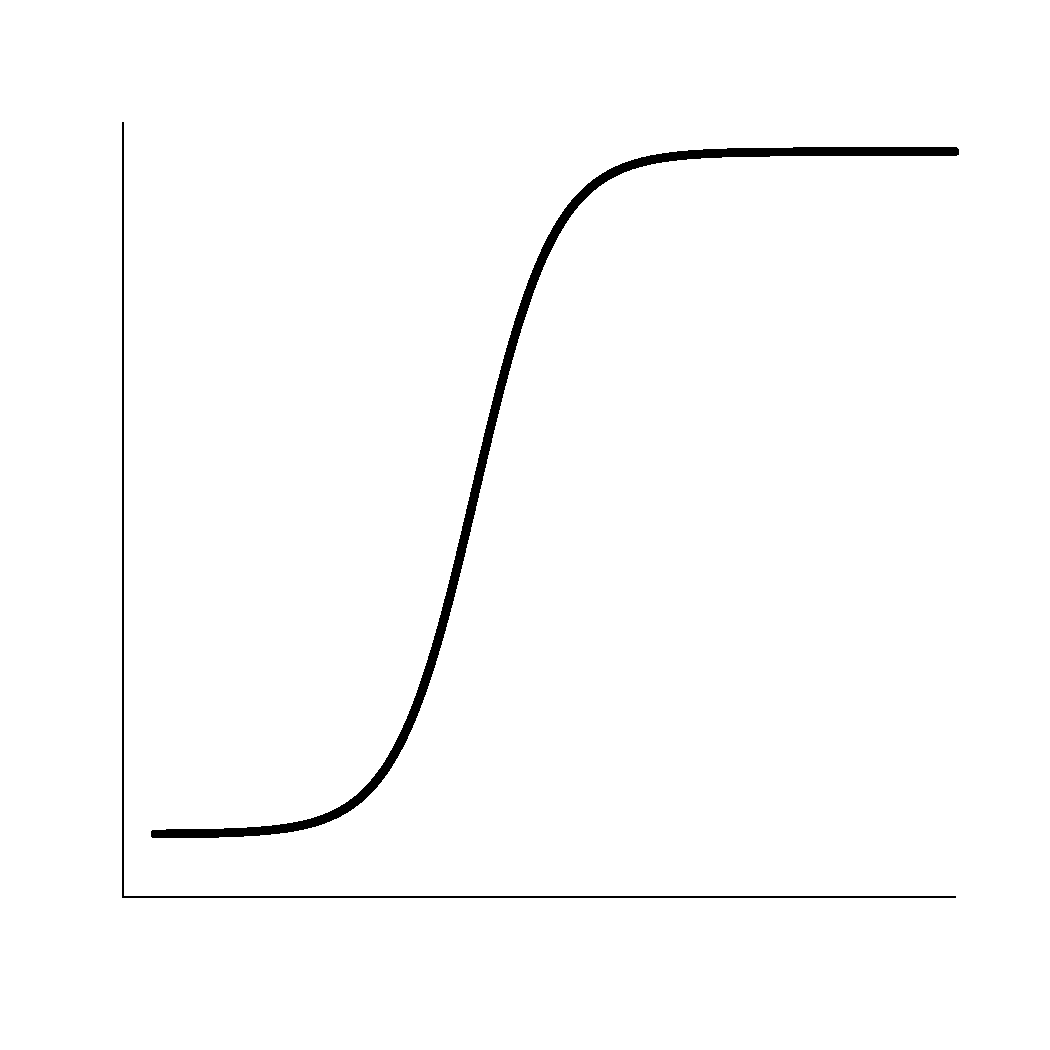
\includegraphics[scale=0.4]{img/logistic_a.pdf}
\end{center}


\end{frame}

\begin{frame}{Onset of look}
\vspace{-5mm}
\begin{center}
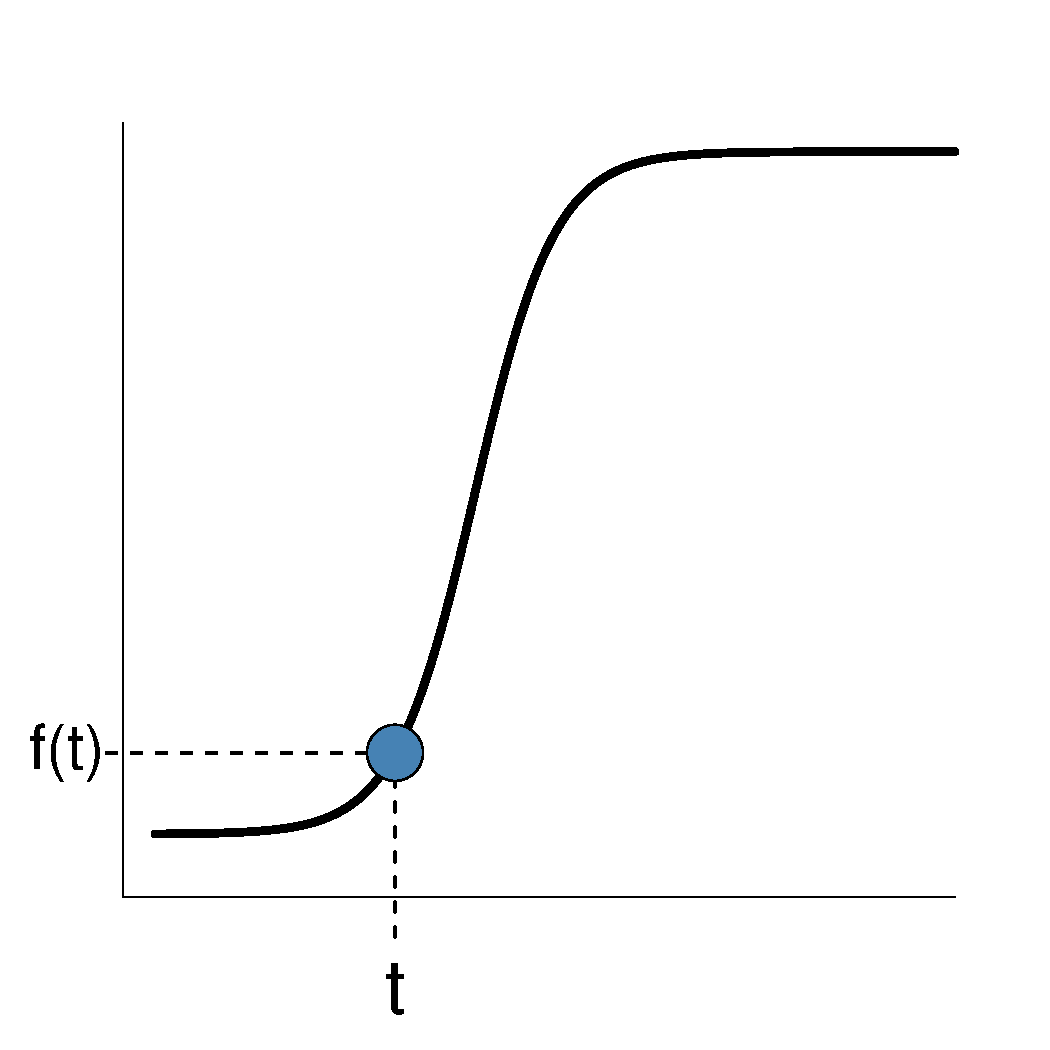
\includegraphics[scale=0.4]{img/logistic_b.pdf}
\end{center}

\end{frame}

\begin{frame}{...followed by fixation}
\vspace{-5mm}
\begin{center}
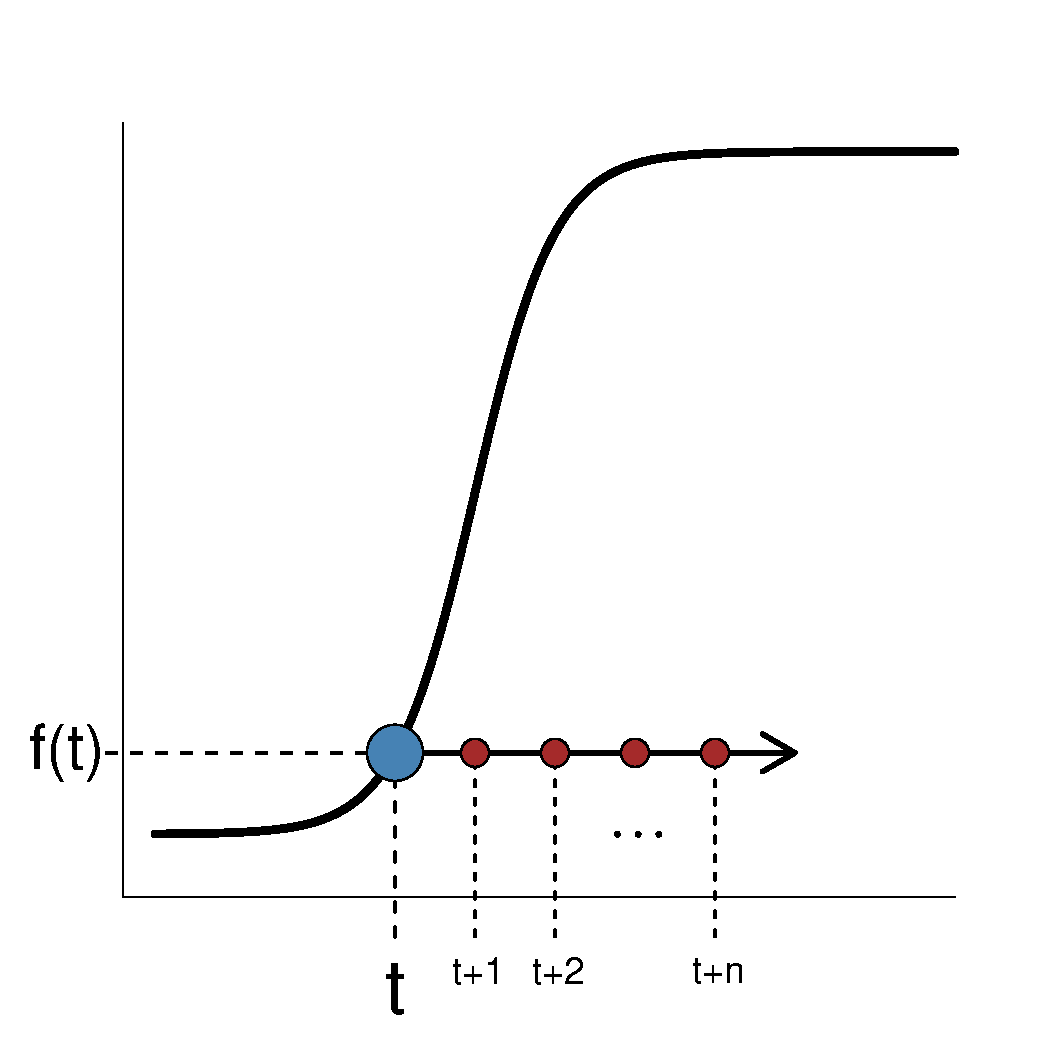
\includegraphics[scale=0.4]{img/logistic_c.pdf}
\end{center}
\end{frame}

\begin{frame}{Look Onset Method}
Only the initial moment of look onset and its location, $s_k$, is considered relevant in the recovery of latent activation, where a look initiated at time $t_k$ follows 
\vspace{-4mm}

\begin{align*}
s_k \sim Bern \left[f(t_k | \theta)\right].
\end{align*}

This gives us instead a set of ordered pairs, $\mathcal{S} = \{(s_k, t_k)\}_{k=1}^K$ rather than a time ordered vector of proportions  \vspace{4mm}

We are able to use an identical procedure as before, 

\begin{align*}
\hat{\theta} = \argmin_{\theta} \mathcal{L}(f_{\theta}, \mathcal{S})
\end{align*}

\end{frame}

\begin{frame}{Look Onset Data}


\begin{columns}
\begin{column}{0.45\textwidth}

\begin{table}[ht]
\centering
\begin{tabular}{cc}
\multicolumn{2}{c}{Look Onset Data} \\ 
& \\
  \hline
$t$ & Target \\ 
  \hline
100 &  0 \\ 
  500 &  0 \\ 
  900 &  1 \\ 
  400 &  0 \\ 
  700 &  1 \\ 
  1400 &  0 \\ 
   \vdots & \vdots \\ 
   800 & 0 \\ 
    1200 &  1 \\
   \hline
\end{tabular}
\end{table}


\end{column}
\begin{column}{0.45\textwidth}  %%<--- here

\begin{table}[ht]
\centering
\begin{tabular}{cc}
\multicolumn{2}{c}{Proportion Data} \\ 
& \\
  \hline
$t$ & Target \\ 
  \hline
  0 & 0.00 \\ 
    4 & 0.01 \\ 
    8 & 0.02 \\ 
   12 & 0.02 \\ 
   16 & 0.04 \\ 
   \vdots & \vdots \\ 
  1596 & 0.91 \\ 
  1600 & 0.92 \\ 
   \hline
\end{tabular}
\end{table}
\end{column}
\end{columns}

\end{frame}



\begin{frame}{Delayed Observation}\large

Between the cognitive mechanism and the initiation of look onset is a period of oculomotor delay, $\rho$ \vspace{4mm}

This gives distribution of look onset,
\vspace{-1mm}
\begin{align*}
s_j \sim Bern \left[f(t_j - \rho) | \theta)\right].
\end{align*}

It is ``roughly" estimated to be around 200ms, and this is typically accounted for by subtracting 200ms from observations \vspace{4mm}

We show that varying degree of randomness in this process have an impact in observed error and successful recovery



\end{frame}



\begin{frame}{Simulation}\large

Create simulated VWP trials with eye mechanics oriented towards Target, the goal of recovering activation curve, $f(t|\theta)$ \vspace{4mm}

Each subject draws individual $\theta_i$ and performs 300 trials \vspace{4mm}

 1,000 total subjects \vspace{4mm}

Estimate generating function using both  methods \vspace{4mm}

Metric for efficacy is MISE between generating and recovered curve
\end{frame}



\begin{frame}{Simulation Mechanics}

\vspace{-2.5mm}
\begin{figure}
\centering
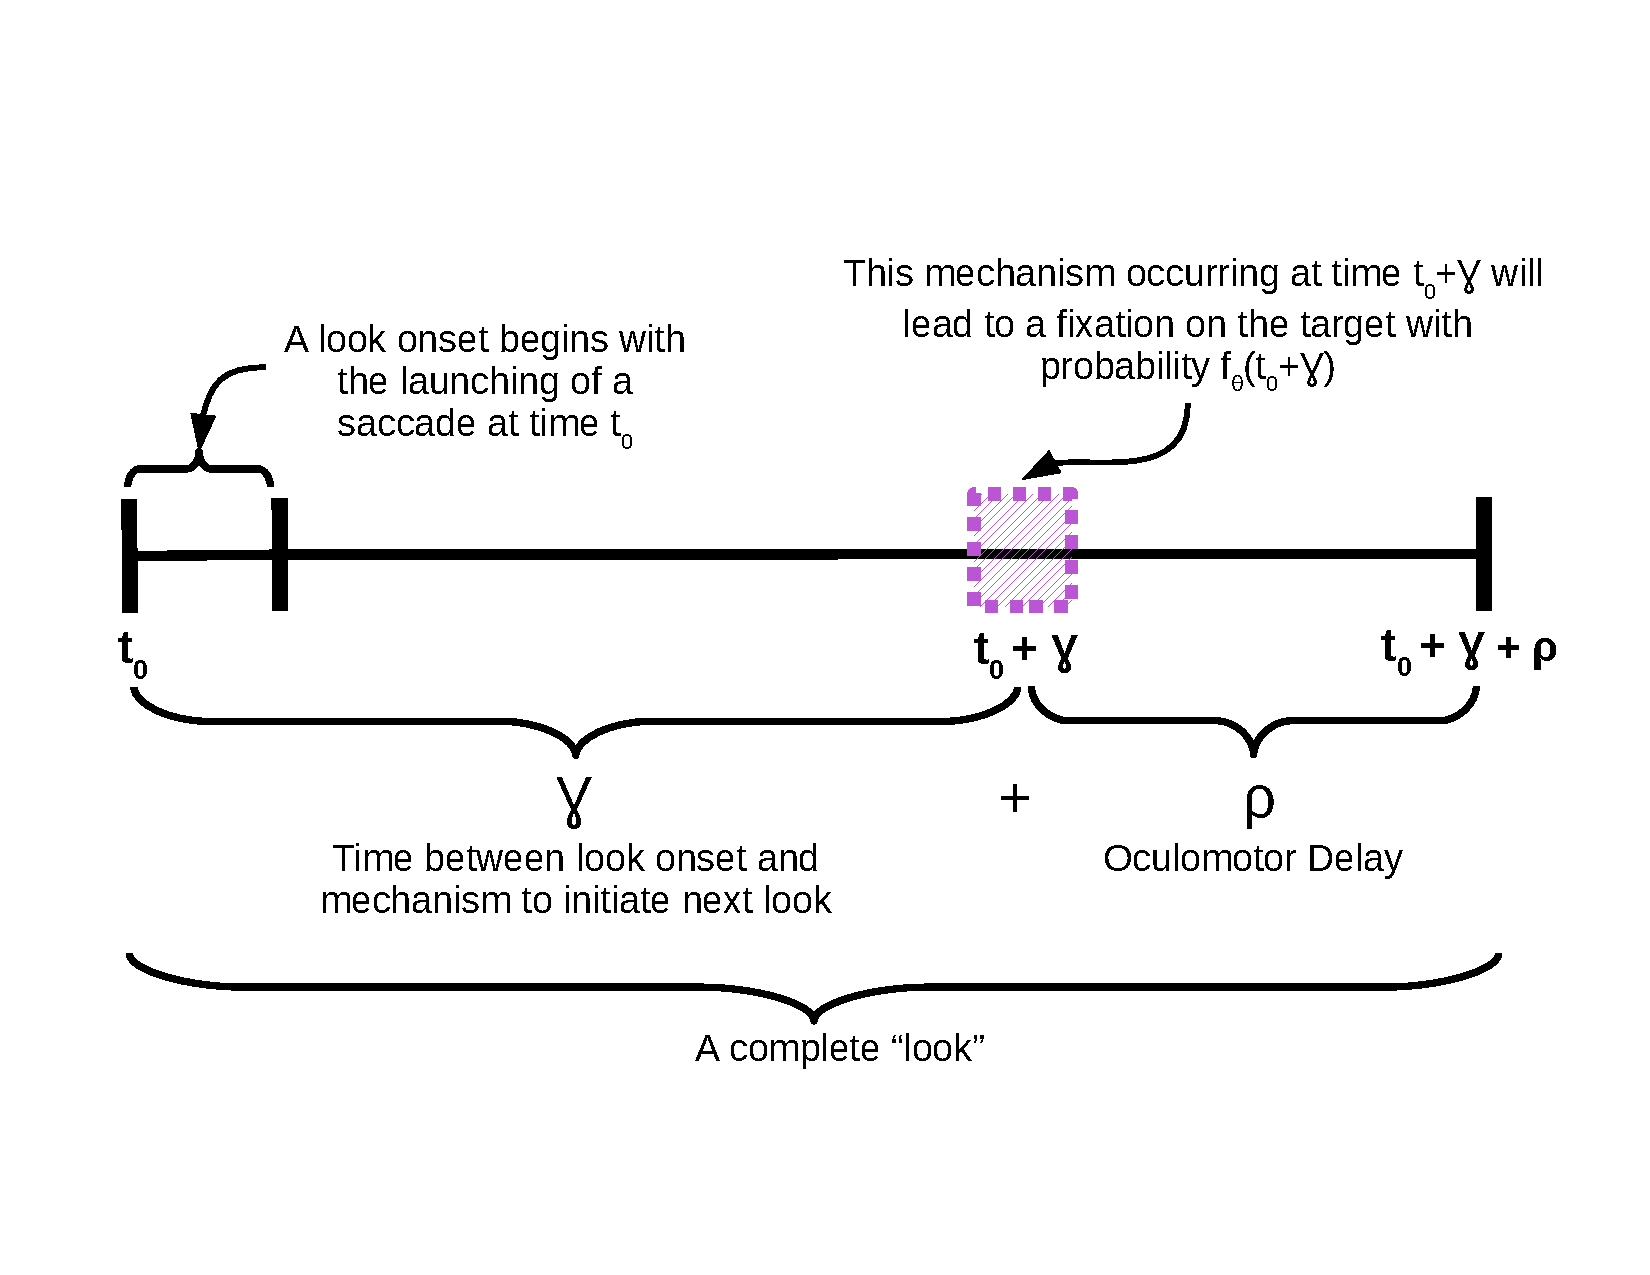
\includegraphics[scale=0.4]{look_comp.pdf}
\end{figure}
\end{frame}




\begin{frame}
\begin{figure}[H]
\centering
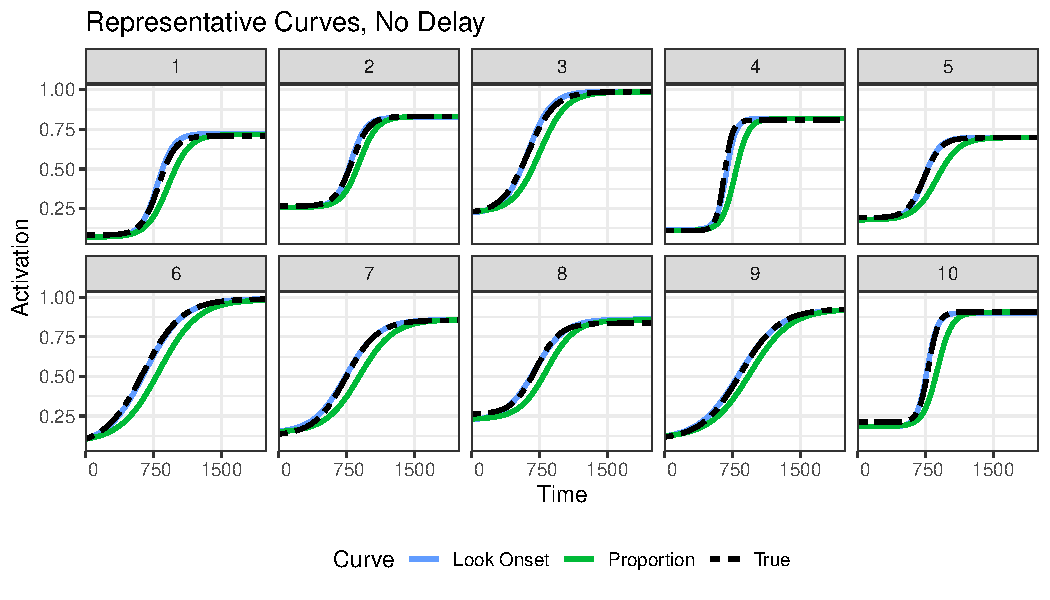
\includegraphics{rep_curves_no_delay.pdf}
\end{figure}
\end{frame}

\begin{frame}
\begin{figure}[H]
\centering
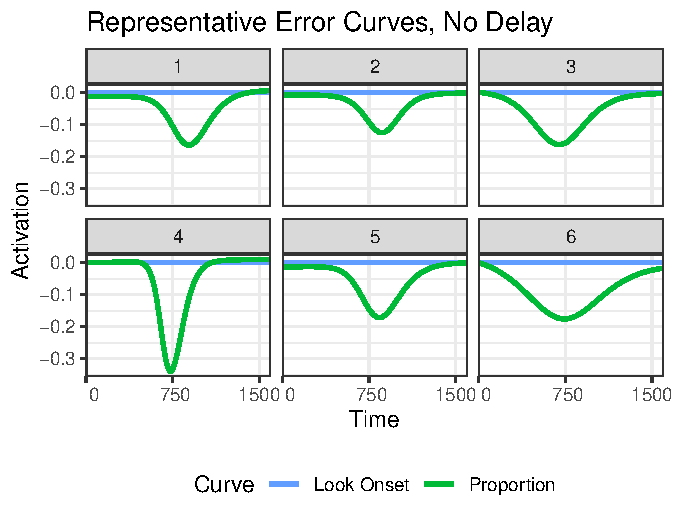
\includegraphics{error_no_delay.pdf}
\end{figure}
\end{frame}


\begin{frame}
\begin{figure}[H]
\centering
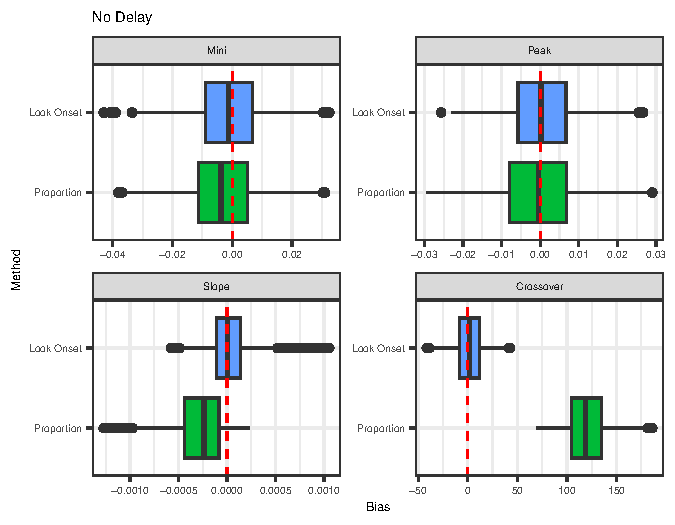
\includegraphics{no_delay_bar_plot.pdf}
\end{figure}
\end{frame}


\begin{frame}
\begin{figure}
\centering
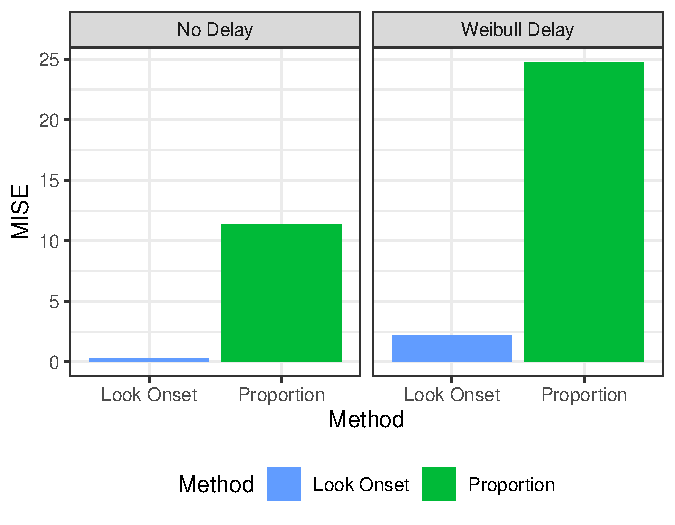
\includegraphics{mise_bar.pdf}
\end{figure}
\end{frame}

\begin{frame}
\begin{figure}[H]
\centering
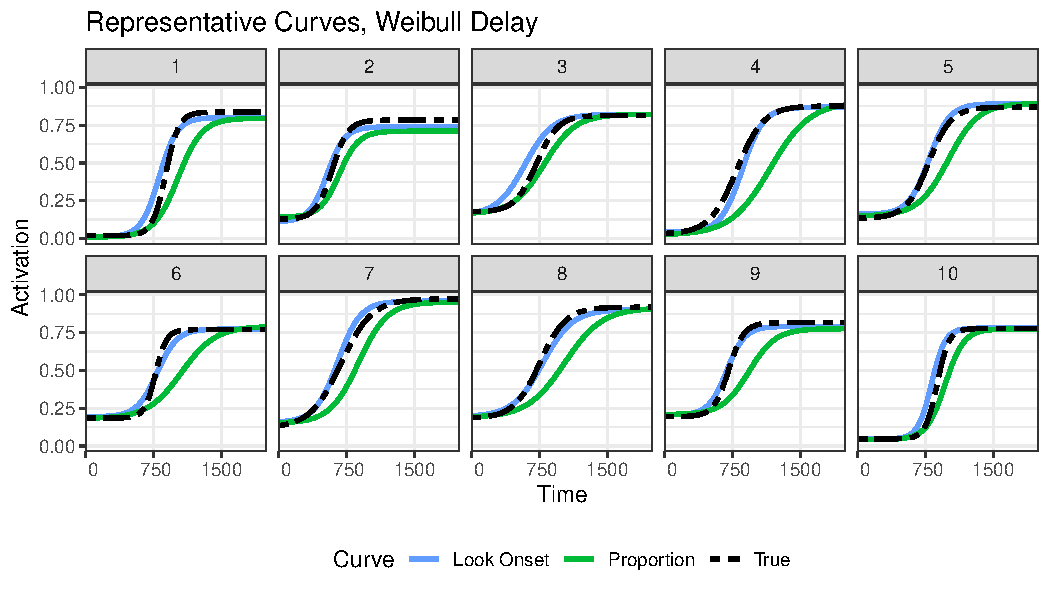
\includegraphics{rep_curves_weibull_delay.pdf}
\end{figure}
\end{frame}

\begin{frame}
\begin{figure}[H]
\centering
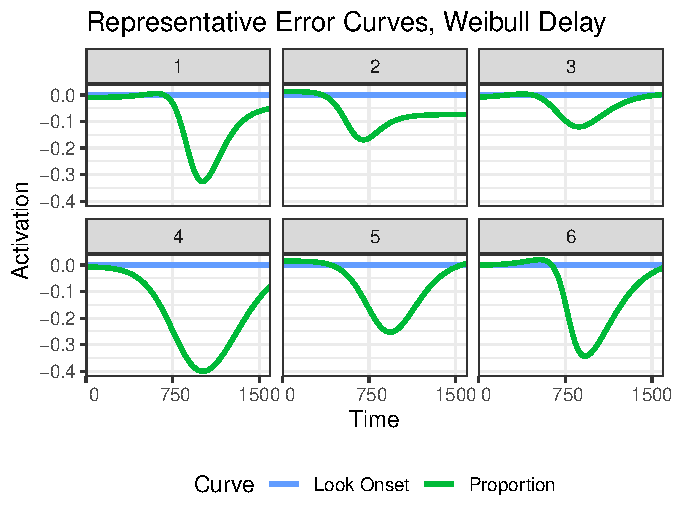
\includegraphics{error_weibull_delay.pdf}
\end{figure}
\end{frame}


%\begin{frame}
%\begin{figure}[H]
%\centering
%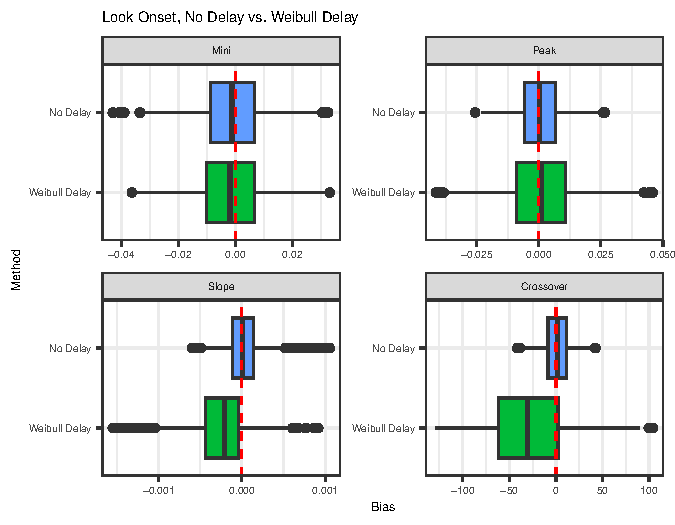
\includegraphics{compare_bar_plot.pdf}
%\end{figure}
%\end{frame}

\begin{frame}
\begin{figure}[H]
\centering
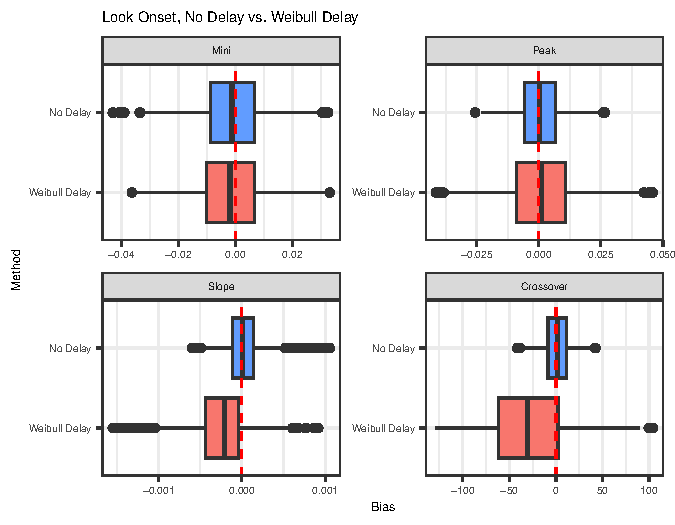
\includegraphics{compare_bar_plot2.pdf}
\end{figure}
\end{frame}

%
%\begin{frame}{MISE}
%\cn{make this bar plot LOL}
%\begin{table}[H]
%\centering
%\begin{tabular}{llrrr}
%  \hline
%Method & Delay & 1st Qu. & Median & 3rd Qu. \\ 
%  \hline
%Look Onset & No Delay & 0.17 & 0.32 & 0.56 \\ 
%  Look Onset & Weibull Delay & 1.05 & 2.16 & 4.23 \\ 
%  Proportion & No Delay & 8.21 & 11.33 & 16.01 \\ 
%  Proportion & Weibull Delay & 15.27 & 24.75 & 38.14 \\ 
%   \hline
%\end{tabular}
%\caption{Summary of mean integrated squared error across simulations}
%\label{tab:mise_sims}
%\end{table}
%
%\end{frame}





%% End with list of other things that I will be doing going forward
\begin{frame}{What else?}

\xt{bdots} package 
\begin{itemize}
\item Significant overhaul to interface
\item Broad expansion of capabilities
\end{itemize}
\vspace{4mm}

Underlying methodology
\begin{itemize}
\item Introduced two new methods
\item Type I Error
\item Power
\end{itemize}

%\begin{itemize}
%\item Rewrote \xt{bdots} package (thanks Seedorff)
%\item Expand and improve upon underlying methodology
%\end{itemize}
\end{frame}




\begin{frame}{Bootstrapped differences in time series -- \texttt{bdots}}
\vspace{-1mm}
\begin{center}
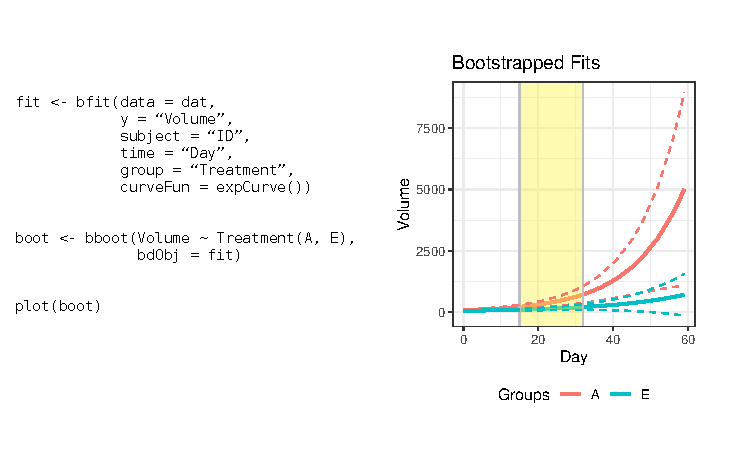
\includegraphics{bdots_examples.pdf}
\end{center}
\end{frame}


\begin{frame}{Methodology}
\vspace{-7mm}
\begin{center}
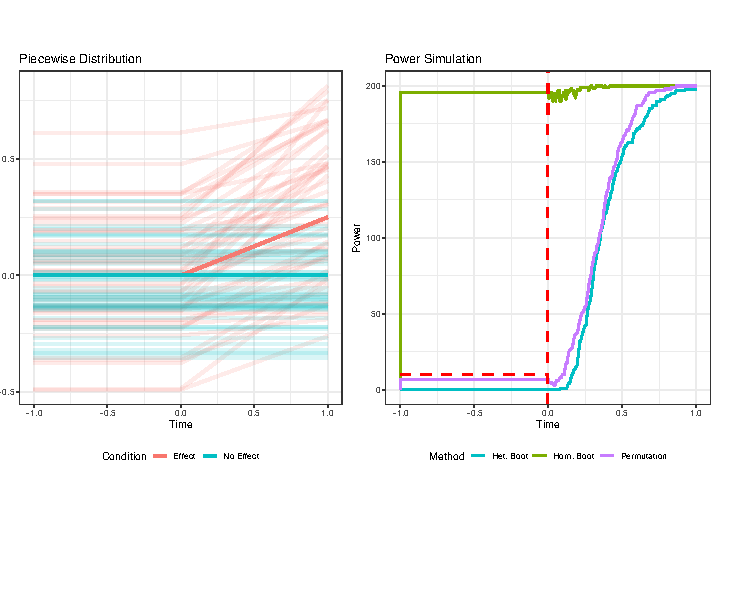
\includegraphics{method_image.pdf}
\end{center}
\end{frame}




\begin{frame}
\centering
thanks
\end{frame}


\begin{frame}{References}\small
Magnuson, James S. \textbf{Fixations in the visual world paradigm: where, when, why?} 2019-09 \textit{Journal of Cultural Cognitive Science}, Vol. 3, No. 2 Springer  Science and Business Media LLC p. 113-139 \newline \\

McMurray, Bob \textbf{I'm not sure that curve means what you think it means: Towards a [more] realistic understanding of the role of eye-movement generation in the visual world paradigm} 2022 \textit{Psychonomic Bulletin \& Review} p 1-45 \newline \\

Oleson, Jacob J; Cavanaugh, Joseph E, McMurray, Bob; Brown, Grant \textbf{Detecting time-specific differences between temporal nonlinear curves: Analyzing data from the visual world paradigm} 2017 \textit{Statistical Methods in Medical Research}, Vol. 26, No. 6 p 2708-2725 \newline \\

Paul D. Allopenna, James S. Magnuson, Michael K. Tanenhaus
\textbf{Tracking the Time Course of Spoken Word Recognition Using Eye Movements: Evidence for Continuous Mapping Models} 1998 \textit{Journal of Memory and Language}, Vol. 38, Issue 4 p 419-439

\end{frame}



\end{document}